\chapter{Endokrinologi dan Homeostasis}\label{ch:b3:endocrinology}

Pada musim panas tahun 1921, dua pemuda di sebuah laboratorium Toronto yang panas
mengikat saluran pankreas beberapa anjing, lalu menunggu jaringan
pencernaannya melayu, menggerus sisanya, lalu menyuntikkan sarinya ke seekor anjing
yang dibuat diabetes dengan membuang pankreasnya. Gula darahnya turun. Pada
bulan Januari, seorang anak lelaki berumur empat belas tahun yang sekarat karena diabetes di Rumah Sakit Umum
Toronto menerima sari itu, dan dalam beberapa minggu ia dapat makan,
berjalan, serta bertambah bobot; ia hidup tiga belas tahun lagi. Zat
itu, yakni \omterm{def:b3:endocrinology:glucose}{insulin}, adalah sebuah peptida beranggota lima puluh satu asam amino yang disekresikan
oleh satu persen pankreasnya ke dalam darah, tempat pada kepekatan
beberapa ratus pikomolar ia memberi tahu tiap sel otot dan lemak di dalam tubuhnya
apa yang harus dilakukan dengan gula santapan terakhirnya. Bab ini tentang
pesuruh semacam itu: apa mereka, bagaimana sebuah sel yang tidak pernah menjumpai kelenjarnya
tahu apa arti pesannya, bagaimana kelenjarnya sendiri diatur
dalam sebuah hierarki gelung umpan balik, dan bagaimana keseluruhan sistemnya menahan
glukosa, garam, kalsium, dan suhu darahnya dalam beberapa persen
seumur hidup --- serta apa yang terjadi, di klinik, ketika salah satu
gelungnya gagal.

\section{Hormon dan reseptornya}

\begin{definition}[Hormon]\label{def:b3:endocrinology:hormone}
\index{hormon}\index{kelenjar endokrin}\index{parakrin}%
\index{hormon steroid}\index{hormon peptida}\index{reseptor inti}
Sebuah \emph{hormon} adalah sebuah zat yang dilepaskan sebuah sel ke dalam darah
yang bekerja pada sel jauh yang mengusung reseptornya; sebuah isyarat \emph{parakrin}
bekerja pada tetangganya, sebuah isyarat \emph{autokrin} pada sel yang
membuatnya, dan sebuah neurohormon dilepaskan sebuah neuron ke dalam darahnya.
\emph{Kelenjar endokrin} klasiknya --- \omterm{def:b3:endocrinology:axes}{hipofisis}, tiroid,
paratiroid, adrenal, pulau pankreas, gonad --- kini bergabung
dengan jantung (peptida natriuretik), ginjal (eritropoietin), lemak
(leptin), usus (selusin peptida), dan tulang. Secara kimia, hormon ada
tiga jenis, dan kimianya memancangkan mekanismenya. \emph{Hormon peptida
dan protein} (\omterm{def:b3:endocrinology:glucose}{insulin}, hormon pertumbuhan, hormon
\omterm{def:b3:endocrinology:axes}{hipofisis}) dibuat pada ribosom, disimpan di dalam butiran, dilepaskan lewat
eksositosis, mengembara bebas di dalam plasmanya, tidak dapat melintasi selaput, lalu bekerja pada
reseptor di permukaan selnya --- tergandeng-protein~G atau terkait-kinase ---
lewat pesuruh kedua, dalam hitungan detik sampai menit; paruh hidupnya
beberapa menit. \emph{Steroid} (kortisol, \omterm{def:b3:renal-osmoregulation:controls}{aldosteron}, estrogen,
testosteron, dan sekosteroid \omterm{def:b3:endocrinology:calcium}{vitamin D}) dibuat dari kolesterol
sesuai keperluan, tidak disimpan, mengembara terikat pada protein pengusung, melintasi
selaput, lalu mengikat \emph{reseptor inti} yang sendirinya
faktor transkripsi: pengaruhnya memakan waktu berjam-jam lalu bertahan berhari-hari.
\emph{Amina} berkangkang di antara keduanya: adrenalin bekerja di permukaan dalam
sedetik; \omterm{prop:b3:endocrinology:thyroid}{hormon tiroidnya}, walaupun turunan asam amino, bekerja pada
reseptor inti seperti steroid. Sebuah hormon tidak berarti apa-apa dengan sendirinya:
adrenalin yang sama melebarkan satu pembuluh lalu menyempitkan pembuluh lain sebab
otot polosnya mengusung subtipe reseptor yang berbeda, dan kortisol yang sama
menaikkan glukosa darah di hati lalu menekan sebuah \omterm{def:b3:adaptive-immunity:lymphocytes}{limfosit} sebab
\omterm{def:b3:chromatin-epigenetics:nucleosome}{kromatin} kedua selnya menawarkan gen yang berbeda kepada reseptornya.
\end{definition}

\begin{omfigure}
\begin{tikzpicture}[every node/.style={font=\scriptsize}, >=stealth]
  % peptide pathway
  \draw[thick, omDef, fill=omDef!10] (0,0) rectangle (5.2,3.4);
  \node[above] at (2.6,3.4) {hormon peptida atau amina --- reseptor permukaan};
  \draw[thick, omDef] (0,2.6) -- (5.2,2.6); \node[left, font=\tiny] at (5.2,2.75) {selaput};
  \node[circle, fill=omThm!60, inner sep=2pt, label={[font=\tiny]0:hormon}] (h1) at (1.4,3.1) {};
  \draw[thick, omDef!80!black, fill=omDef!40] (1.1,2.3) rectangle (1.7,2.9); \node[below, font=\tiny] at (1.4,2.3) {reseptor};
  \draw[->, thick] (2.0,2.1) -- (3.0,2.1) node[right, align=left, font=\tiny] {protein G atau\\keaktifan kinase};
  \draw[->, thick] (2.6,1.75) -- (2.6,1.25) node[below, align=center, font=\tiny] {cAMP, Ca$^{2+}$, IP$_3$, atau\\runtunan fosforilasi};
  \draw[->, thick] (2.6,0.55) -- (2.6,0.25) node[below=-2pt, font=\tiny] {enzim dinyalakan: detik sampai menit};
  % steroid pathway
  \draw[thick, omProp, fill=omProp!10] (6.4,0) rectangle (11.6,3.4);
  \node[above] at (9.0,3.4) {hormon steroid atau tiroid --- reseptor inti};
  \draw[thick, omProp] (6.4,2.6) -- (11.6,2.6);
  \node[circle, fill=omMeth!70, inner sep=2pt, label={[font=\tiny]0:hormon pada pengusung}] (h2) at (7.6,3.1) {};
  \draw[->, thick] (7.6,2.95) -- (7.6,2.2) node[below, font=\tiny] {membaur menembusnya};
  \draw[->, thick] (7.9,1.85) -- (9.0,1.5); \draw[thick, omProp!80!black, fill=omProp!35] (8.8,1.0) rectangle (9.6,1.7); \node[right, align=left, font=\tiny] at (9.65,1.35) {kompleks hormon--reseptor,\\yakni sebuah\\faktor transkripsi};
  \draw[thick, omProp] (7.0,0.2) rectangle (11.0,0.8); \node[font=\tiny] at (9.0,0.5) {inti: gen hidup atau mati --- jam sampai hari};
  \draw[->, thick] (9.2,1.0) -- (9.2,0.82);
\end{tikzpicture}

{\small Dua cara mendengar sebuah \omterm{def:b3:endocrinology:hormone}{hormon}. \omterm{def:b3:endocrinology:hormone}{Hormon} yang larut air berhenti di
permukaan lalu bekerja lewat pesuruh kedua, dengan cepat dan singkat; \omterm{def:b3:endocrinology:hormone}{hormon} yang
larut lipid masuk, mengikat sebuah reseptor yang merupakan faktor transkripsi, lalu mengubah
apa yang dibuat selnya, dengan lambat dan lama.}
\end{omfigure}

\begin{proposition}[Dosis dan tanggapan]\label{prop:b3:endocrinology:dose}
\index{kurva dosis--tanggapan}\index{reseptor cadangan}\index{penurunan pengaturan}
Sebuah sel dengan $R$ reseptor bertetapan disosiasi $K_{d}$ di dalam sebuah
kepekatan \omterm{def:b3:endocrinology:hormone}{hormon} $H$ punya $R\,H/(K_{d} + H)$ di antaranya yang terhuni, dan
tanggapannya biasanya naik seiring penghuniannya sepanjang sebuah sigmoid pada sebuah
sumbu dosis logaritma, setengah maksimal pada sebuah $\text{EC}_{50}$ yang
kerap jauh di bawah $K_{d}$: penghunian beberapa persen memberi sebuah tanggapan
penuh, sebab isyaratnya dilipatgandakan di hilirnya (satu reseptor
mengaktifkan banyak protein G, satu kinase memfosforilasi banyak
substrat), dan \emph{\omterm{prop:b3:endocrinology:dose}{reseptor cadangan}} yang berlebih itu menggeser kurvanya
ke kiri lalu membuat selnya peka pada dosis rendah. Selnya menala
kepekaannya sendiri: pemaparan yang lama pada sebuah \omterm{def:b3:endocrinology:hormone}{hormon} menyingkirkan
reseptornya dari permukaannya (\emph{\omterm{prop:b3:endocrinology:dose}{penurunan pengaturan}}), yakni mekanisme yang
dengannya \omterm{def:b3:endocrinology:glucose}{insulin} yang terus-menerus tinggi menumpulkan pengaruh \omterm{def:b3:endocrinology:glucose}{insulin} itu sendiri;
kekurangannya menambahnya. \omterm{def:b3:endocrinology:hormone}{Hormon} beredar pada $10^{-12}$ sampai
$10^{-9}$ molar --- seribu sampai sejuta kali di bawah kebanyakan
metabolit --- dan itulah sebabnya reseptornya harus mengikatnya dengan
afinitas nanomolar, serta sebabnya mengukurnya memerlukan sebuah cara baru.
\end{proposition}
\begin{proof}
Penghuniannya adalah isoterm aksi massa sebuah tapak pengikat tunggal. Bila
tanggapannya menjenuh ketika $n \ll R$ reseptor terhuni, maka ia
setengah maksimal ketika $R H/(K_{d} + H) = n/2$, yakni $H = K_{d}\,
(n/2)/(R - n/2) \approx K_{d}\, n/(2R) \ll K_{d}$: EC$_{50}$-nya jatuh
sebanding dengan kelebihan reseptornya. Kehilangan reseptor menaikkannya,
dan itulah pengaruh \omterm{prop:b3:endocrinology:dose}{penurunan pengaturan} pada kurvanya.
\end{proof}

\begin{method}[Radioimunouji]\label{met:b3:endocrinology:ria}
\index{radioimunouji}\index{imunouji}
Untuk mengukur sebuah \omterm{def:b3:endocrinology:hormone}{hormon} pada kepekatan pikomolar (Yalow dan Berson,
1959): (1) bangkitkanlah sebuah \omterm{def:b3:adaptive-immunity:antibody}{antibodi} terhadapnya; (2) campurkanlah sejumlah kecil tetap
\omterm{def:b3:adaptive-immunity:antibody}{antibodinya} dengan sejumlah tetap \omterm{def:b3:endocrinology:hormone}{hormon} berlabel radioaktif,
lalu tambahkanlah contohnya; (3) \omterm{def:b3:endocrinology:hormone}{hormon} tak berlabel contohnya bersaing
dengan yang berlabel memperebutkan tapak \omterm{def:b3:adaptive-immunity:antibody}{antibodinya}, sehingga makin banyak \omterm{def:b3:endocrinology:hormone}{hormon} yang
dimuat contohnya, makin sedikit label yang terikat; (4) pisahkanlah label yang terikat dari yang
bebas lalu cacahlah; (5) bacalah kepekatan contohnya pada sebuah kurva
baku yang dibuat dengan jumlah yang diketahui. Keturunannya mengganti isotopnya
dengan sebuah enzim atau sebuah fluorofor lalu memakai dua \omterm{def:b3:adaptive-immunity:antibody}{antibodi} (sebuah ``roti lapis'')
untuk memperoleh kekhasan; mereka mengukur tiap \omterm{def:b3:endocrinology:hormone}{hormon} di dalam bab ini dari
setetes darah, dan menjadikan endokrinologi sebuah ilmu kuantitatif.
\end{method}

\section{Hierarkinya: hipotalamus dan hipofisis}

\begin{definition}[Porosnya]\label{def:b3:endocrinology:axes}
\index{hipotalamus}\index{hipofisis}\index{sistem portal}%
\index{hormon pelepas}\index{hormon tropik}\index{umpan balik negatif}
\emph{Hipotalamus}, beberapa gram otak di atas hipofisisnya,
mengubah keterangan saraf --- tekanan, dingin, panjang hari, \omterm{def:b3:renal-osmoregulation:problem}{osmolaritas} dan
glukosa darahnya --- menjadi perintah hormonal. Sel
neurosekretorinya melepaskan \emph{\omterm{def:b3:endocrinology:hormone}{hormon} pelepas} (peptida:
CRH, TRH, GnRH, GHRH, dan penghambatnya somatostatin; dopamin bagi
prolaktin) ke dalam sebuah \emph{sistem portal} pembuluh yang
mengusungnya, tanpa terencerkan, sesentimeter turun ke \emph{hipofisis
depan}, yang selnya menjawab dengan \emph{\omterm{def:b3:endocrinology:hormone}{hormon} tropik}: ACTH ke
korteks adrenalnya, TSH ke tiroidnya, LH dan FSH ke gonadnya,
\omterm{def:b3:endocrinology:hormone}{hormon} pertumbuhan ke hati dan jaringannya, prolaktin ke payudaranya. \omterm{def:b3:endocrinology:hormone}{Hormon}
kelenjar sasarannya --- kortisol, tiroksin, steroid kelamin ---
mengumpan balik pada hipofisis dan hipotalamusnya untuk mematikan perintahnya
sendiri: itulah \emph{umpan balik negatif}, dalam tiga tingkat.
\emph{Hipofisis belakang} bukanlah sebuah kelenjar melainkan terminal akson
neuron hipotalamusnya, yang melepaskan vasopresin dan oksitosin langsung ke dalam
darahnya. Tiap porosnya punya dinamikanya sendiri: poros tiroidnya lambat
dan mantap, yang menahan sebuah \omterm{thm:b3:endocrinology:loop}{titik setel} bertahun-tahun; poros adrenalnya
berdenyut dan sirkadia, dengan kortisolnya memuncak sebelum fajar lalu disekresikan dalam
ledakan tiap jam; poros gonad seorang perempuan menjalankan sebuah daur bulanan pada
sebuah umpan balik positif yang tidak dipunyai poros lain.
\end{definition}

\begin{omfigure}
\begin{tikzpicture}[every node/.style={font=\scriptsize}, >=stealth]
  \node[draw, thick, rounded corners, fill=omDef!20, align=center, minimum width=3.2cm] (hyp) at (0,3.4) {hipotalamus\\CRH, TRH, GnRH, GHRH};
  \node[draw, thick, rounded corners, fill=omDef!20, align=center, minimum width=3.2cm] (pit) at (0,1.7) {hipofisis depan\\ACTH, TSH, LH/FSH, GH};
  \node[draw, thick, rounded corners, fill=omProp!25, align=center, minimum width=3.2cm] (gl) at (0,0) {kelenjar sasaran\\kortisol, T$_4$, steroid kelamin};
  \node[draw, thick, rounded corners, fill=omMeth!25, align=center, minimum width=3.2cm] (tis) at (0,-1.7) {jaringan: pengaruhnya};
  \draw[->, very thick] (hyp) -- (pit) node[midway, right, font=\tiny] {pembuluh portal};
  \draw[->, very thick] (pit) -- (gl) node[midway, right, font=\tiny] {darah};
  \draw[->, very thick] (gl) -- (tis);
  \draw[-|, thick, omThm] (gl.west) -- ++(-0.9,0) |- (pit.west) node[pos=0.25, left, font=\tiny, omThm, align=right] {gelung\\pendek};
  \draw[-|, thick, omThm] (gl.west) ++(-0.9,0) -- ++(-0.7,0) |- (hyp.west) node[pos=0.25, left, font=\tiny, omThm, align=right] {gelung\\panjang};
  \node[left, align=right, font=\tiny] at (-2.0,4.4) {masukan: tekanan, dingin,\\cahaya, metabolit};
  \draw[->, thick] (-1.9,4.3) -- (hyp.north west);
  % right: the thyroid example with numbers
  \node[right, align=left] at (3.4,3.4) {poros tiroid: TRH $\to$ TSH $\to$ T$_4$, T$_3$;\\paruh hidup T$_4$ 7 hari, titik setelnya tertahan lama;\\log TSH turun linear seiring naiknya T$_4$ bebas};
  \node[right, align=left] at (3.4,1.7) {poros adrenal: CRH $\to$ ACTH $\to$ kortisol;\\denyut tiap 1--2 j, puncaknya sebelum bangun;\\tekanan mengatasi umpan baliknya};
  \node[right, align=left] at (3.4,0) {poros gonad: denyut GnRH $\to$ LH, FSH $\to$\\estradiol, progesteron, testosteron;\\sebuah lonjakan umpan balik positif sebulan sekali};
  \node[right, align=left] at (3.4,-1.7) {poros pertumbuhan: GHRH, somatostatin $\to$ GH $\to$\\IGF-1 dari hatinya; denyut pada malam hari};
\end{tikzpicture}

{\small Poros tiga tingkatnya. \omterm{def:b3:endocrinology:axes}{Hormon pelepas} mencapai \omterm{def:b3:endocrinology:axes}{hipofisisnya}
lewat pembuluh portalnya; \omterm{def:b3:endocrinology:axes}{hipofisisnya} memerintah sebuah kelenjar; \omterm{def:b3:endocrinology:hormone}{hormon}
kelenjarnya mematikan kedua tingkat di hulunya. Tiap porosnya punya iramanya sendiri dan
kegagalannya sendiri.}
\end{omfigure}

\begin{proof}[Bukti eksperimental]
Berthold (1849) mengebiri ayam jantan muda, yang lalu kehilangan jenggernya, kokoknya, dan
sifat suka berkelahinya; menanamkan kembali sebuah testis di mana pun di dalam perutnya, tanpa
sarafnya, memulihkannya --- organnya bekerja lewat darahnya. Harris
(dasawarsa 1950-an) memotong pembuluh portal antara \omterm{def:b3:endocrinology:axes}{hipotalamus} dan \omterm{def:b3:endocrinology:axes}{hipofisis} pada
tikus: \omterm{def:b3:endocrinology:axes}{hipofisisnya}, yang pasokan darahnya dipulihkan dari tempat lain, berhenti
menanggapi tekanan dan indung telurnya berhenti berdaur; mencangkokkan sebuah
\omterm{def:b3:endocrinology:axes}{hipofisis} di bawah ginjalnya membiarkannya lembam, tetapi di bawah \omterm{def:b3:endocrinology:axes}{hipotalamusnya},
tempat pembuluh portalnya tumbuh kembali ke dalamnya, ia bekerja --- otaknya mengatur
kelenjarnya lewat faktor yang diusung darah, lalu Guillemin dan Schally mengasingkan
yang pertama di antaranya, yakni TRH, dari jutaan \omterm{def:b3:endocrinology:axes}{hipotalamus} domba dan babi
(1969): tiga asam amino.
\end{proof}

\begin{proposition}[Umpan balik dan tiroid log-linear]\label{prop:b3:endocrinology:thyroid}
\index{hormon tiroid}\index{TSH}\index{hipotiroidisme}%
\index{hipertiroidisme}\index{gondok}
Tiroidnya mengambil iodida, lalu membuat tiroksin T$_{4}$ (empat
iodin), yang diubah jaringannya menjadi T$_{3}$ yang aktif; keduanya menaikkan
laju metabolisme nyaris tiap selnya, menetapkan denyut jantungnya, dan
diperlukan bagi perkembangan otak sebelum dan sesudah lahir. TSH dari
\omterm{def:b3:endocrinology:axes}{hipofisisnya} menggerakkan baik sintesis maupun pertumbuhan kelenjarnya; T$_{4}$
menekan TSH. Hubungannya pada keadaan mantap bersifat \emph{log-linear}: yakni
logaritma TSH turun sebanding dengan T$_{4}$ bebasnya,
\[
\text{TSH} = \text{TSH}_{0}\,\mathrm{e}^{-\kappa\,(T_{4} - T_{4,0})},
\]
sehingga sebuah penurunan T$_{4}$ bebas sebesar sepertiga menaikkan TSH sekitar sepuluh kali lipat ---
dan itulah sebabnya TSH, dan bukan T$_{4}$, yang menjadi uji yang peka: sebuah kelenjar yang
mulai gagal menunjukkan T$_{4}$ yang normal yang ditahan tetap tinggi oleh TSH yang sudah beberapa
kali normal. Kegagalan kelenjarnya (pemusnahan autoimun, kekurangan
iodin) memberi \emph{hipotiroidisme} --- dingin, lambat, lelah, dengan
TSH yang tinggi dan, pada kekurangan iodin, sebuah kelenjar yang membesar menjadi sebuah
\emph{gondok} oleh TSH yang tidak dapat membuatnya menghasilkan; sebuah \omterm{def:b3:adaptive-immunity:antibody}{antibodi} yang
meniru TSH memberi \emph{hipertiroidisme} (penyakit Graves) dengan seorang pasien yang panas,
cepat, dan kurus serta sebuah TSH yang tertekan menjadi nol, sebab
rangsangannya lolos dari umpan baliknya. Seorang bayi baru lahir tanpa \omterm{prop:b3:endocrinology:thyroid}{hormon tiroid}
mengembangkan disabilitas intelektual yang tak terpulihkan dalam beberapa bulan, dan itulah
sebabnya TSH tiap bayi baru lahir diukur pada setitik darah.
\end{proposition}
\begin{proof}
Keluaran TSH sel \omterm{def:b3:endocrinology:axes}{hipofisisnya} menanggapi penghunian reseptornya oleh
T$_{3}$, yang sendirinya sebanding dengan T$_{4}$, dan tanggapan sebuah
penekanan transkripsi terhadap sebuah perubahan penghuniannya bersifat perkalian
--- tiap pertambahan \omterm{def:b3:endocrinology:hormone}{hormonnya} menekan pecahan yang sama dari apa yang
tersisa --- sehingga $\mathrm{d}\ln\text{TSH}/\mathrm{d}T_{4} = -\kappa$,
yang darinya eksponensialnya berasal. Dengan $\kappa$ yang dicocokkan sehingga $T_{4}$ yang turun
dari $15$ ke \qty{10}{pmol/L} menaikkan TSH dari $1.5$ ke \qty{15}{mU/L},
$\kappa = \ln 10/5 = \qty{0.46}{L/pmol}$: TSH berlipat dua tiap
\qty{1.5}{pmol/L} T$_{4}$ yang hilang, yakni pelipatgandaan yang menjadikannya
uji yang peka.
\end{proof}

\begin{omfigure}
\begin{tikzpicture}
\begin{semilogyaxis}[
  width=0.6\linewidth, height=5.6cm,
  axis x line=bottom, axis y line=left,
  xmin=4, xmax=30, ymin=0.02, ymax=200,
  xlabel={T$_4$ bebas (pmol/L)}, ylabel={TSH (mU/L)},
  xlabel style={font=\small, at={(axis description cs:0.5,-0.12)}, anchor=north}, ylabel style={font=\small},
  tick label style={font=\small}, xtick={5,10,15,20,25,30}, ytick={0.1,1,10,100},
  yticklabels={0.1,1,10,100},
  clip=false,
]
\addplot[very thick, omDef, domain=4.5:24.4, samples=60] {1.5*exp(-0.46*(x-15))};
\fill[omProp, opacity=0.15] (axis cs:10,0.4) rectangle (axis cs:20,4);
\node[font=\scriptsize, omProp!80!black, anchor=south] at (axis cs:15,4.2) {jangkauan acuan};
\node[font=\scriptsize, omThm, anchor=north west, align=left] at (axis cs:12,150) {kelenjar yang gagal:\\TSH tinggi, T$_4$ masih normal};
\node[font=\scriptsize, omMeth!70!black, anchor=south west, align=left] at (axis cs:22,0.5) {penyakit Graves:\\T$_4$ tinggi, TSH tertekan};
\end{semilogyaxis}
\end{tikzpicture}

{\small \omterm{thm:b3:endocrinology:loop}{Titik setel} tiroidnya yang dilihat dari luar. Karena log TSH turun
linear seiring T$_4$, sebuah penurunan kecil \omterm{def:b3:endocrinology:hormone}{hormonnya} menghasilkan kenaikan besar
perintahnya --- \omterm{def:b3:endocrinology:axes}{hipofisisnya} adalah sebuah pelipat ganda logaritma bagi
kegagalan kelenjarnya.}
\end{omfigure}

\begin{example}[Kortisol: poros tekanan]\label{ex:b3:endocrinology:cortisol}
Kortisol, dari korteks adrenal di bawah ACTH, menyiagakan bahan bakar (glukosa
dari hatinya, asam amino dari ototnya, asam lemak dari lemaknya),
memekakan pembuluhnya terhadap adrenalin, serta menekan \omterm{def:b3:innate-immunity:inflammation}{peradangan} dan
tanggapan imunnya --- yakni alasan kerabat sintetisnya menjadi
obat antiradang yang terlazim. Iramanya ditetapkan jamnya:
\qty{500}{nmol/L} pada pukul 8 pagi, seperlimanya pada tengah malam, dan denyut
tiap satu atau dua jam sepanjang waktu, sebab neuron CRH \omterm{def:b3:endocrinology:axes}{hipotalamusnya} menyala
dalam ledakan. Tekanan --- pendarahan, infeksi, pembedahan, ketakutan --- menaikkannya
sepuluh kali lipat dalam hitungan menit, yang mengatasi umpan baliknya. Terlalu sedikit (penyakit
Addison, yakni pemusnahan korteks adrenalnya) memberi kelemahan, tekanan darah
rendah, glukosa rendah, dan, di bawah tekanan, kolaps serta kematian kecuali
diganti; terlalu banyak (sindrom Cushing: sebuah \omterm{def:b3:cancer-biology:hallmarks}{tumor} \omterm{def:b3:endocrinology:axes}{hipofisis} yang membuat ACTH,
sebuah \omterm{def:b3:cancer-biology:hallmarks}{tumor} adrenal, atau, paling sering, steroid yang diresepkan) memberi wajah
bulat, kulit tipis, otot yang menyusut, glukosa tinggi, tekanan tinggi, serta tulang
rapuh dari pemaparan yang lama. Menghentikan sebuah pengobatan steroid yang panjang
secara mendadak berbahaya karena alasan yang diramalkan porosnya: \omterm{def:b3:endocrinology:axes}{hipotalamus} dan
\omterm{def:b3:endocrinology:axes}{hipofisis} yang tertekan memakan waktu berminggu-minggu untuk pulih, dan adrenalnya,
yang tak terangsang, telah menyusut.
\end{example}

\begin{omfigure}
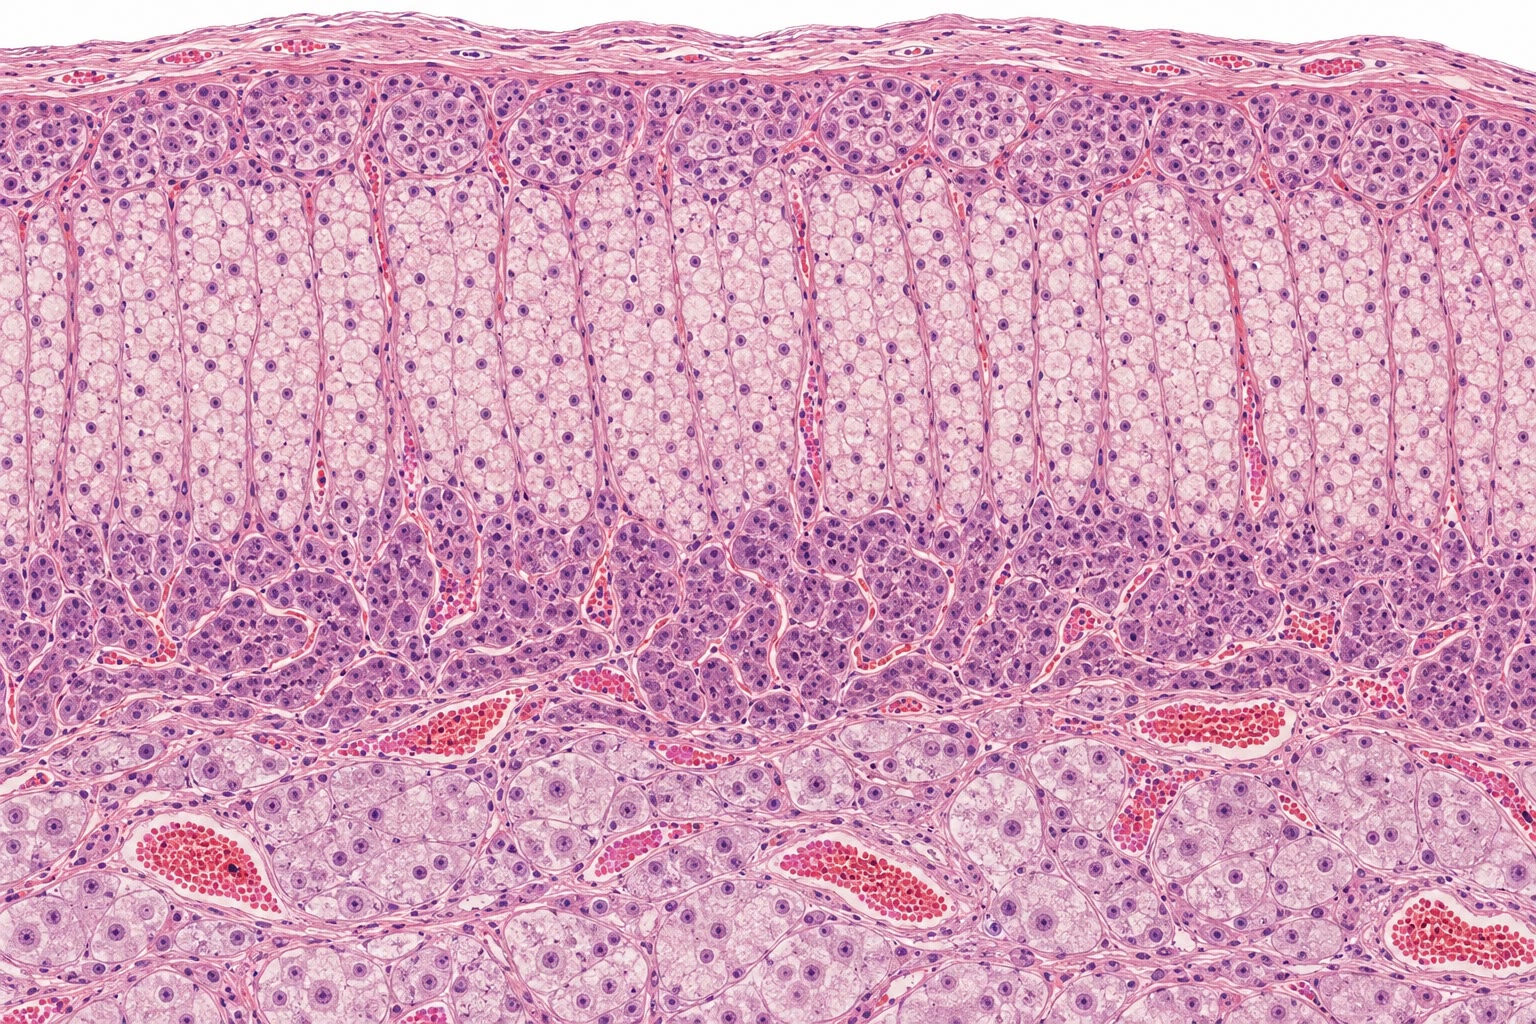
\includegraphics[width=0.5\linewidth]{images/book5/ai/b5-21-adrenal-section.jpg}\hspace{0.04\linewidth}
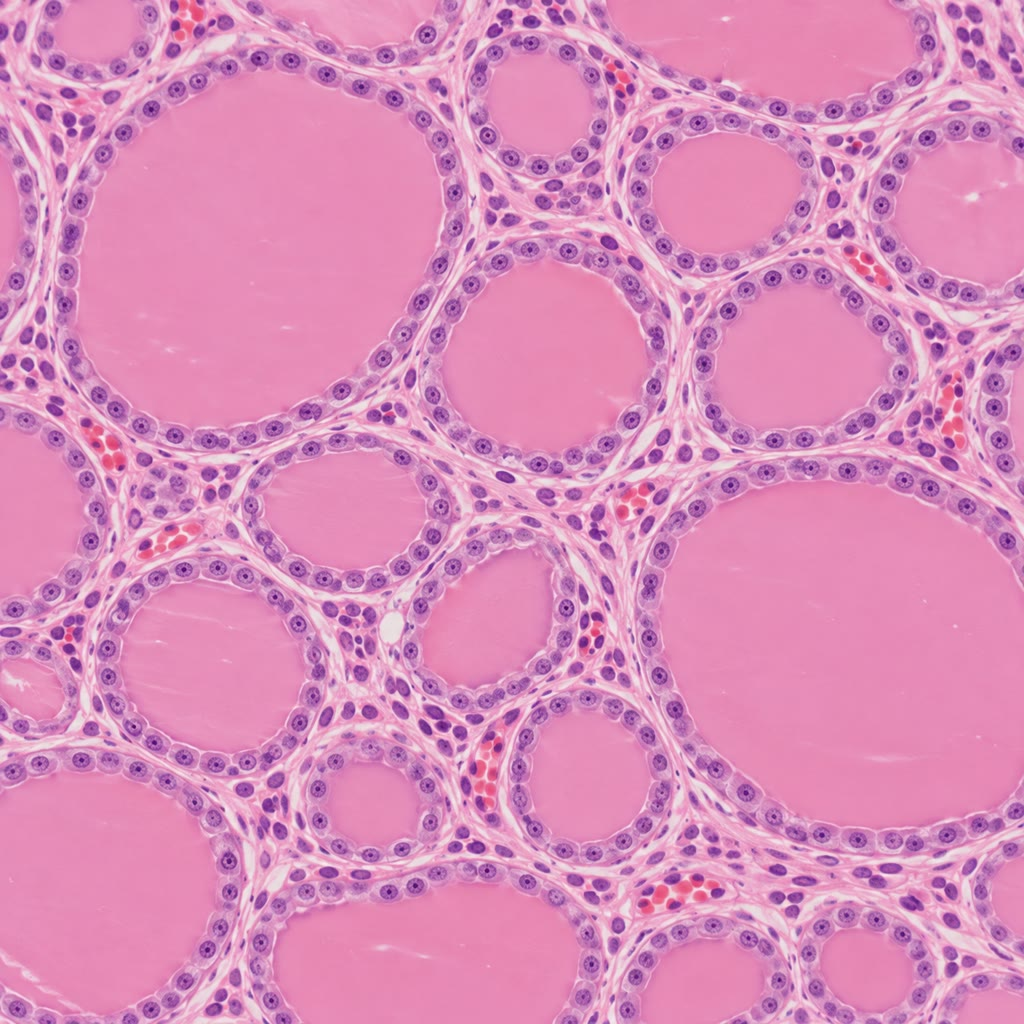
\includegraphics[width=0.36\linewidth]{images/book5/ai/b5-21-thyroid-follicles.jpg}

{\small Kiri: kelenjar adrenal dalam irisan --- korteksnya dalam ketiga
zonanya (\omterm{def:b3:renal-osmoregulation:controls}{aldosteron} terluar, kortisol di zona tengah yang lebar,
androgen terdalam) di sekeliling sebuah medula berisi sel kromafin penyekresi adrenalin,
yang menurut asalnya sebuah \omterm{def:b3:nervous-systems:comparative}{ganglion} simpatis. Kanan:
folikel tiroid, masing-masing sebuah bola sel di sekeliling sebuah simpanan koloid
yang memuat \omterm{def:b3:endocrinology:hormone}{hormon} senilai berbulan-bulan yang terikat pada tiroglobulin.}
\end{omfigure}

\section{Glukosa: gelung yang terketat}

\begin{definition}[Insulin dan glukagon]\label{def:b3:endocrinology:glucose}
\index{insulin}\index{glukagon}\index{pulau Langerhans}%
\index{GLUT4}\index{diabetes melitus}
Darahnya memuat sekitar \qty{5}{g} glukosa, pada \qty{5}{mmol/L}
(\qty{90}{mg/dL}), dan otaknya membakar \qty{120}{g} tiap hari lalu tidak dapat membakar
apa pun yang lain; sebuah santapan menghantarkan \qty{75}{g} dalam sejam.
\emph{Pulau Langerhans}, yakni sejuta gugusan berisi beberapa ribu sel yang
tersebar di seluruh pankreasnya, memegang gelungnya. Sel $\beta$ mengindera
glukosanya dengan memetabolismekannya: makin banyak glukosa, makin banyak ATP, menutupnya
sebuah saluran kalium peka-ATP, depolarisasi, masuknya kalsium, dan
eksositosis \emph{insulin}, yakni sebuah \omterm{def:b3:endocrinology:hormone}{hormon peptida} yang dipotong dari sebuah pendahulu
tunggal. Insulin memberi tahu otot dan lemaknya untuk memindahkan pengangkut
\emph{GLUT4} ke permukaannya lalu mengambil glukosanya, hatinya untuk menyimpan
glukosa sebagai glikogen dan berhenti membuatnya, dan lemaknya untuk berhenti melepaskan asam
lemak: ia \omterm{def:b3:endocrinology:hormone}{hormon} keadaan kenyang, satu-satunya yang menurunkan
glukosa darahnya. Sel $\alpha$ melepaskan \emph{glukagon} ketika glukosanya
turun: hatinya merombak glikogennya lalu membuat glukosa baru dari asam
amino dan laktat. Adrenalin, kortisol, dan \omterm{def:b3:endocrinology:hormone}{hormon} pertumbuhan menaikkan
glukosanya pula, dan kelebihannya tidak setangkup: sebuah tubuh dapat bertahan
terhadap sebuah penurunan lewat empat jalan dan terhadap sebuah kenaikan lewat satu jalan. \emph{Diabetes
melitus} adalah kegagalan satu jalan itu: jenis 1, yakni pemusnahan autoimun
sel $\beta$-nya, memerlukan insulin sejak hari pertama;
jenis 2, yakni sembilan dari sepuluh kasusnya, bermula sebagai kekebalan jaringannya terhadap
insulin, yang ditemui bertahun-tahun dengan lebih banyak insulin, sampai sel $\beta$-nya gagal
mengimbanginya dan glukosanya naik.
\end{definition}

\begin{theorem}[Gelung insulin--glukosa]\label{thm:b3:endocrinology:loop}
\index{bati gelung}\index{titik setel}\index{ayunan teredam}
Tulislah $g$ dan $i$ bagi simpangan glukosa dan \omterm{def:b3:endocrinology:glucose}{insulin} plasma dari
nilai puasanya. Glukosanya dibersihkan pada sebuah laju yang sebanding dengan
kelebihannya sendiri (yakni kemangkusan glukosa $a$) dan dengan kelebihan \omterm{def:b3:endocrinology:glucose}{insulinnya}
(kepekaan $s$); \omterm{def:b3:endocrinology:glucose}{insulinnya} disekresikan sebanding dengan kelebihan
glukosanya ($\beta$) lalu dibersihkan pada laju $\gamma$; sebuah muatan $u$ masuk:
\[
\dot g = -a\,g - s\,i + u, \qquad \dot i = \beta\,g - \gamma\,i .
\]
Di bawah sebuah muatan tetap $u$, glukosanya menetap pada
\[
g^{*} = \frac{u}{a}\cdot\frac{1}{1 + L}, \qquad L = \frac{s\beta}{a\gamma},
\]
sehingga umpan baliknya membagi gangguan yang akan diderita sebuah tubuh
tak terkendali dengan $1 + L$, yakni \emph{\omterm{thm:b3:endocrinology:loop}{bati gelung}}-nya ditambah satu. Sesudah sebuah bolus,
kembalinya diatur nilai eigennya
$\lambda = -\tfrac{a + \gamma}{2} \pm \sqrt{\tfrac{(a+\gamma)^{2}}{4} - (a\gamma + s\beta)}$:
monoton bila $s\beta < (a - \gamma)^{2}/4$, dan jika tidak sebuah \omterm{thm:b3:endocrinology:loop}{ayunan
teredam} berfrekuensi sudut $\omega = \sqrt{a\gamma + s\beta -
(a+\gamma)^{2}/4}$ yang meluruh sebagai $\mathrm{e}^{-(a+\gamma)t/2}$ --- glukosanya
menembus ke bawah nilai puasanya sebelum menetap, yakni
hipoglikemia ringan dua atau tiga jam sesudah sebuah santapan bergula. Kekebalan
\omterm{def:b3:endocrinology:glucose}{insulin} menurunkan $s$: keadaan mantap puasanya di bawah keluaran hati tubuhnya
sendiri naik, dan gelungnya mengimbangi dengan $i^{*}$ yang lebih tinggi
sampai $\beta$ sel $\beta$-nya turun pula, ketika imbangannya gagal.
\end{theorem}
\begin{proof}
Keadaan mantapnya: $\dot i = 0$ memberi $i^{*} = \beta g^{*}/\gamma$; dengan menaruhnya
di dalam $\dot g = 0$: $a g^{*} + s\beta g^{*}/\gamma = u$, yang darinya $g^{*} =
u/(a + s\beta/\gamma) = (u/a)/(1 + L)$. Dinamikanya: matriks sistemnya adalah
$\begin{pmatrix} -a & -s\\ \beta & -\gamma\end{pmatrix}$, dengan jumlah diagonal
$-(a+\gamma)$ dan determinan $a\gamma + s\beta$; persamaan cirinya
$\lambda^{2} + (a+\gamma)\lambda + (a\gamma + s\beta) = 0$ punya
akar yang dinyatakan. Keduanya berbagian nyata negatif, sehingga keadaan puasanya
mantap; akarnya kompleks ketika diskriminannya $(a+\gamma)^{2}
- 4(a\gamma + s\beta) = (a-\gamma)^{2} - 4s\beta$ negatif, yakni
syarat yang diberikan, dan lalu $g(t) = \mathrm{e}^{-(a+\gamma)t/2}(A\cos\omega t
+ B\sin\omega t)$, yang melintasi nol. Kekebalannya: dengan $u$ adalah keluaran
basal hatinya dan $s$ yang berkurang, $L$ turun dan $g^{*}$ naik bagi $u$ yang sama;
$i^{*} = \beta g^{*}/\gamma$ naik bersamanya (hiperinsulinemia);
bila $\beta$ lalu turun, $L$ turun lebih jauh dan $g^{*}$ mendaki ke arah $u/a$.
\end{proof}

\begin{omfigure}
\begin{tikzpicture}
\begin{axis}[
  width=0.58\linewidth, height=5.6cm,
  axis x line=bottom, axis y line=left,
  xmin=0, xmax=180, ymin=40, ymax=200,
  xlabel={menit sesudah sebuah bolus glukosa}, ylabel={glukosa plasma (mg/dL)},
  xlabel style={font=\small, at={(axis description cs:0.5,-0.12)}, anchor=north}, ylabel style={font=\small},
  tick label style={font=\small}, xtick={0,30,60,90,120,150,180}, ytick={60,90,120,150,180},
  clip=false,
]
\addplot[very thick, omDef, smooth] coordinates {(0,190) (6,165) (12,131) (18,102) (24,84) (30,77) (36,78) (42,82) (48,86) (54,89) (60,91) (66,92) (72,91) (78,91) (84,90) (90,90) (96,90) (102,90) (108,90) (114,90) (120,90) (126,90) (132,90) (138,90) (144,90) (150,90) (156,90) (162,90) (168,90) (174,90) (180,90)};
\draw[dashed, gray] (axis cs:0,90) -- (axis cs:180,90);
\node[font=\scriptsize, gray, anchor=south east] at (axis cs:180,91) {aras puasa};
\node[font=\scriptsize, omDef, anchor=west, align=left] at (axis cs:75,150) {model: $a = \qty{0.02}{min^{-1}}$, $\gamma = \qty{0.1}{min^{-1}}$,\\$s\beta = \qty{0.01}{min^{-2}}$, bati gelung $L = 5$;\\tembusan bawah pada \qty{32}{min}, kala \qty{68}{min}};
\node[font=\scriptsize, omThm, anchor=north] at (axis cs:24,70) {tembusan bawah};
\end{axis}
\begin{axis}[
  at={(0.6\linewidth,0)}, anchor=south west,
  width=0.33\linewidth, height=5.6cm,
  axis x line=bottom, axis y line=left,
  xmin=0, xmax=180, ymin=0, ymax=40,
  xlabel={menit}, ylabel={insulin plasma (mU/L)},
  xlabel style={font=\small, at={(axis description cs:0.5,-0.12)}, anchor=north}, ylabel style={font=\small},
  tick label style={font=\small}, xtick={0,60,120,180}, ytick={0,10,20,30,40},
]
\addplot[very thick, omProp, smooth] coordinates {(0,10.0) (6,30.0) (12,33.7) (18,28.5) (24,20.4) (30,13.4) (36,8.9) (42,7.1) (48,7.1) (54,7.9) (60,9.0) (66,9.8) (72,10.2) (78,10.4) (84,10.4) (90,10.2) (96,10.1) (102,10.0) (108,10.0) (114,9.9) (120,10.0) (126,10.0) (132,10.0) (138,10.0) (144,10.0) (150,10.0) (156,10.0) (162,10.0) (168,10.0) (174,10.0) (180,10.0)};
\draw[dashed, gray] (axis cs:0,10) -- (axis cs:180,10);
\end{axis}
\end{tikzpicture}

{\small Gelung linearnya sesudah sebuah bolus yang menaikkan glukosanya sebesar
\qty{100}{mg/dL}. \omterm{def:b3:endocrinology:glucose}{Insulinnya} memuncak dalam sepuluh menit dan glukosanya kembali
ke dasarnya dalam dua puluh menit, lalu menembus ke bawah; sebuah umpan balik kuat yang bekerja
lewat sebuah \omterm{def:b3:endocrinology:hormone}{hormon} dengan waktu pembersihannya sendiri kembali sebagai sebuah \omterm{thm:b3:endocrinology:loop}{ayunan
teredam} alih-alih sebuah peluruhan sederhana.}
\end{omfigure}

\begin{proof}[Bukti eksperimental]
Von Mering dan Minkowski (1889) membuang pankreas seekor anjing lalu menghasilkan
diabetes --- lalat yang berkerumun pada kemihnya membocorkan gulanya; mengikat
salurannya, yang memusnahkan jaringan pencernaannya tetapi meluputkan pulaunya,
tidak. Banting dan Best (1921), dengan pemurnian Collip, memetik
asas pulaunya lalu menurunkan gula darah seekor anjing diabetes, lalu
gula darah Leonard Thompson (Januari 1922). Sanger mengurutkan \omterm{def:b3:endocrinology:glucose}{insulin} (1955),
yakni urutan protein yang pertama; Yalow dan Berson mengukurnya di dalam darah
(1959) lalu menemukan bahwa penderita diabetes yang bermula pada usia dewasa mula-mula punya lebih banyak
daripada yang sehat --- yakni kekebalan, bukan kekurangan. Bakteri Genentech
membuat \omterm{def:b3:endocrinology:glucose}{insulin} manusia pada tahun 1978, yakni obat rekombinan yang pertama.
\end{proof}

\begin{omfigure}
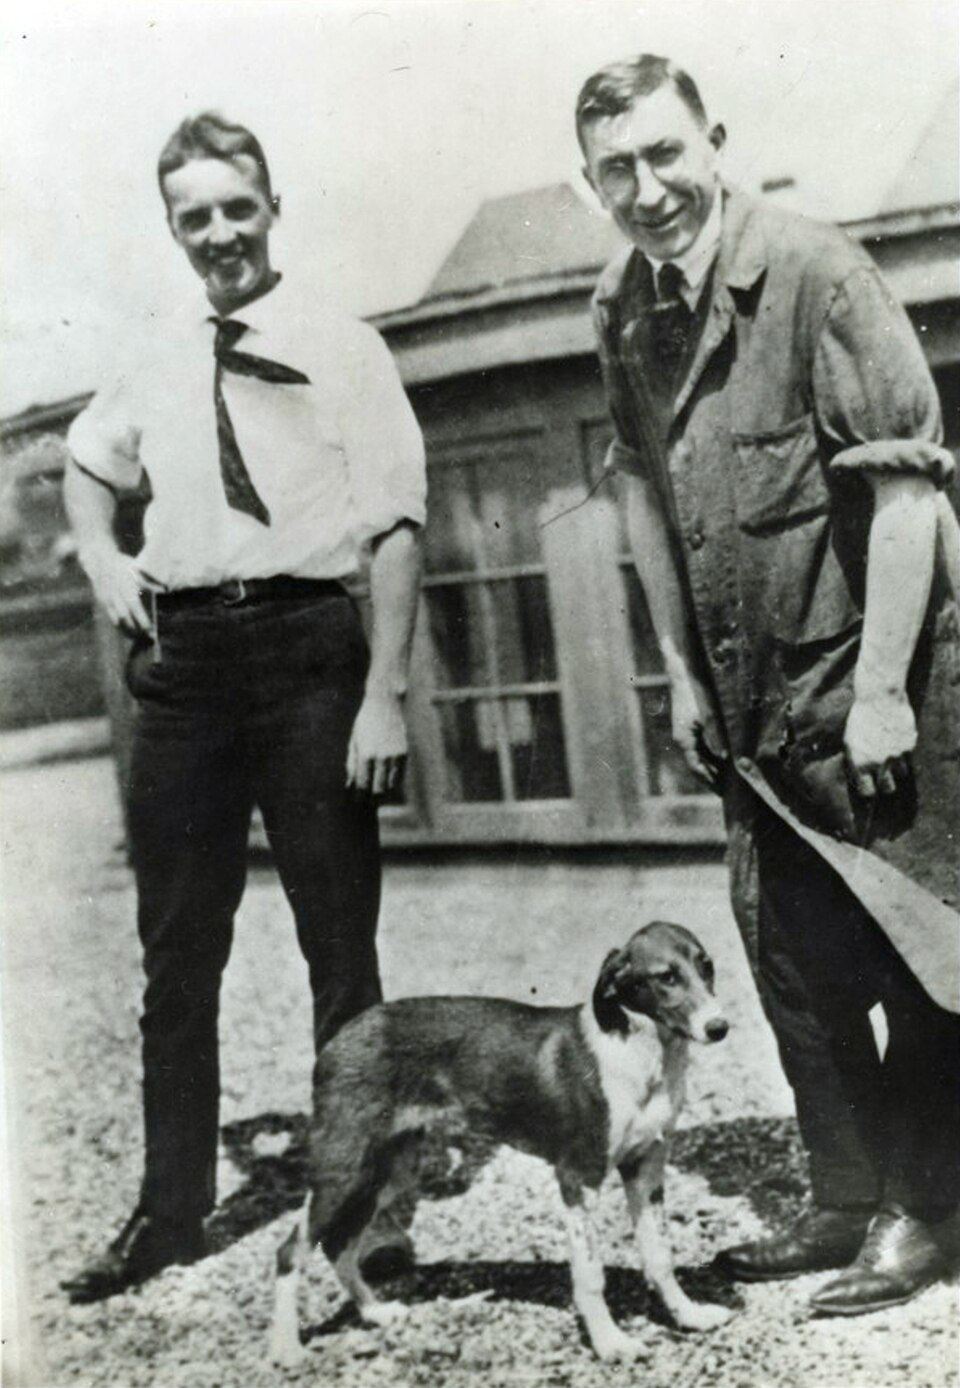
\includegraphics[width=0.42\linewidth]{images/book5/banting-best.jpg}\hspace{0.04\linewidth}
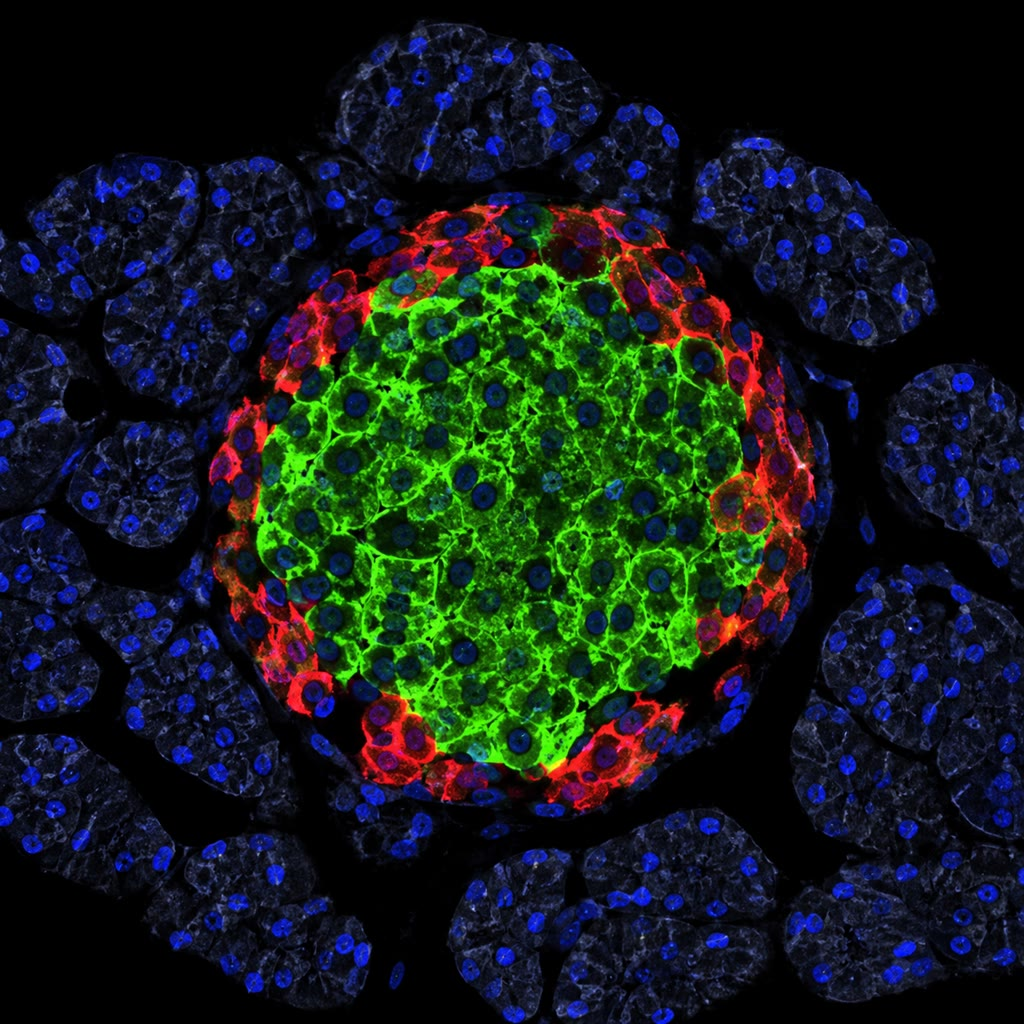
\includegraphics[width=0.42\linewidth]{images/book5/ai/b5-21-pancreatic-islet.jpg}

{\small Kiri: Frederick Banting dan Charles Best di atap gedung
kedokteran di Toronto, sekitar tahun 1924, dengan salah satu anjing percobaan
\omterm{def:b3:endocrinology:glucose}{insulinnya} (foto dalam domain publik). Kanan: sebuah \omterm{def:b3:endocrinology:glucose}{pulau
Langerhans}, dengan sel $\beta$ penghasil \omterm{def:b3:endocrinology:glucose}{insulin} di intinya, sel $\alpha$
\omterm{def:b3:endocrinology:glucose}{glukagon} di tepinya, di dalam sebuah lautan asinus eksokrin.}
\end{omfigure}

\begin{method}[Membaca gelung glukosa pada seorang pasien]\label{met:b3:endocrinology:ogtt}
\index{uji toleransi glukosa}\index{HbA1c}
(1) Glukosa plasma puasa: normal di bawah \qty{5.6}{mmol/L}, diabetes pada
atau di atas \qty{7.0}{mmol/L} pada dua kesempatan. (2) \omterm{met:b3:endocrinology:ogtt}{Uji toleransi glukosa}
lewat mulut: \qty{75}{g} glukosa diminum; glukosa plasma pada dua jam normal
di bawah \qty{7.8}{mmol/L}, diabetes pada atau di atas \qty{11.1}{mmol/L} ---
nilai dua jamnya membaca \omterm{thm:b3:endocrinology:loop}{bati gelungnya}, nilai puasanya \omterm{thm:b3:endocrinology:loop}{titik setelnya}.
(3) Hemoglobin terglikasi, \emph{HbA1c}: glukosanya melekat
secara tak terpulihkan pada hemoglobinnya pada sebuah laju yang sebanding dengan
kepekatannya, dan sel merahnya hidup 120 hari, sehingga pecahan yang terglikasi
mengintegralkan glukosa rata-rata tiga bulan terakhirnya tanpa sebuah puasa
--- normal di bawah \qty{5.7}{\%}, diabetes sejak \qty{6.5}{\%}. (4) Untuk
memisahkan kekebalan dari kekurangan, ukurlah \omterm{def:b3:endocrinology:glucose}{insulinnya} (atau hasil
sampingnya C-peptida) berdampingan: \omterm{def:b3:endocrinology:glucose}{insulin} tinggi dengan glukosa tinggi adalah
kekebalan; C-peptida yang tak ada adalah jenis~1.
\end{method}

\section{Kalsium, dan jamnya}

\begin{definition}[Homeostasis kalsium]\label{def:b3:endocrinology:calcium}
\index{hormon paratiroid}\index{kalsitriol}\index{vitamin D}\index{osteoporosis}
Kalsium terionkan di dalam plasmanya ditahan pada \qty{1.2}{mmol/L} dalam beberapa
persen, sebab ia menetapkan keterangsangan tiap saraf dan ototnya: terlalu
rendah dan mereka menyala dengan sendirinya (tetani), terlalu tinggi dan mereka
lamban. Keempat kelenjar paratiroidnya menginderanya dengan sebuah reseptor permukaan
lalu menyekresikan \emph{\omterm{def:b3:endocrinology:hormone}{hormon} paratiroid} (PTH) sepanjang sebuah sigmoid terbalik
yang curam: PTH menyiagakan kalsium dari tulangnya, membuat ginjalnya menyerapnya kembali
dan mengekskresikan fosfat, lalu mengaktifkan \emph{vitamin D} --- yang dibuat di kulitnya
oleh cahaya ultraungu atau dimakan, dihidroksilasi di hatinya, lalu di ginjalnya
menjadi \emph{kalsitriol} --- yang membuat ususnya menyerap kalsium. Tulangnya adalah
wadahnya, sekilogram kalsium, yang dirombak ulang terus-menerus oleh
osteoklas dan osteoblas di bawah PTH, kalsitriol, estrogen, dan beban.
Kekurangan vitamin D memberi riketsia pada anak dan tulang lunak pada
orang dewasa; turunnya estrogen pada menopause memiringkan perombakan ulangnya ke arah
penyerapan kembali lalu memberi \emph{osteoporosis}; sebuah adenoma paratiroid menaikkan
kalsiumnya, melarutkan tulangnya, lalu membentuk batu ginjal --- ``tulang, batu,
erangan, dan keluhan.''
\end{definition}

\begin{definition}[Jam sirkadia]\label{def:b3:endocrinology:clock}
\index{jam sirkadia}\index{inti suprakiasma}\index{gen jam}%
\index{melatonin}\index{zeitgeber}
Nyaris tiap sel mengusung sebuah \emph{jam sirkadia}: sebuah
gelung transkripsi--terjemahan yang di dalamnya protein CLOCK dan BMAL1
menyalakan gen \emph{Per} dan \emph{Cry}, yang proteinnya
menimbun, memasuki intinya sesudah sebuah penundaan berjam-jam, lalu menekan
transkripsinya sendiri, lalu dirombak, yang melepaskan penekanannya --- satu
daur dalam sekitar dua puluh empat jam, yang ditetapkan laju penundaan dan
perombakannya. Jam tubuhnya diselaraskan sebuah jam induk
berisi dua puluh ribu neuron di dalam \emph{inti suprakiasma}
\omterm{def:b3:endocrinology:axes}{hipotalamusnya}, yang sendirinya disetel cahaya lewat sebuah kelas khusus
\omterm{def:b3:sensory-systems:retina}{sel ganglion} \omterm{def:b3:sensory-systems:retina}{retina} (yang memuat melanopsin, bukan pigmen \omterm{def:b3:sensory-systems:retina}{sel batang} atau
\omterm{def:b3:sensory-systems:retina}{sel kerucutnya}), dan yang mengisyaratkan malam kepada tubuhnya lewat
\emph{melatonin} kelenjar pinealnya, yang disekresikan hanya dalam gelap. Jamnya
menjadwalkan kortisol sebelum bangun, suhu tubuh terendah pada pukul 4 pagi,
\omterm{def:b3:endocrinology:hormone}{hormon} pertumbuhan pada tidur pertama, kepekaan \omterm{def:b3:endocrinology:glucose}{insulin} lebih tinggi pada
pagi hari; makanan, olahraga, dan suhu adalah \emph{zeitgeber}
sekunder yang dapat menarik jam tepinya menjauh dari jam
pusatnya, yakni rasa tak enak pekerja giliran dan pelancong yang lelah terbang ---
sebuah jam hati pada satu waktu dan sebuah jam otak pada waktu lain.
\end{definition}

\begin{proof}[Bukti eksperimental]
Konopka dan Benzer (1971) menyaring lalat mutan mencari irama kemunculan
yang berubah lalu menemukan tiga alel satu gen, yakni \emph{per}: sebuah hari
pendek (19 j), sebuah hari panjang (29 j), dan tanpa irama sama sekali --- yakni sebuah jam dengan
sebuah kala genetik. Hardin, Hall, dan Rosbash (1990) menemukan bahwa
mRNA dan protein \emph{per} berayun dengan sebuah keterlambatan di antaranya, dan
bahwa proteinnya menekan gennya sendiri: itulah gelungnya. Ralph dan Menaker
(1990) mencangkokkan \omterm{def:b3:endocrinology:clock}{inti suprakiasma} seekor hamster mutan berirama
20 jam ke dalam seekor hamster normal yang intinya sendiri telah
dimusnahkan: penerimanya berjalan pada 20 jam --- kalanya milik
jaringan yang dicangkokkan. Pada manusia yang disimpan di dalam sebuah bungker tanpa isyarat waktu,
iramanya berjalan bebas pada sedikit di atas 24 jam; sebuah cahaya terang pada
malam hari menundanya, pada pagi hari memajukannya.
\end{proof}

\begin{omfigure}
\begin{tikzpicture}[every node/.style={font=\scriptsize}, >=stealth]
  \node[draw, thick, rounded corners, fill=omDef!20, align=center] (cb) at (0,1.6) {pengaktif\\CLOCK--BMAL1};
  \node[draw, thick, rounded corners, fill=omProp!25, align=center] (pc) at (3.6,1.6) {\emph{Per}, \emph{Cry}\\ditranskripsi};
  \node[draw, thick, rounded corners, fill=omThm!20, align=center] (pr) at (3.6,-0.4) {protein PER, CRY\\menimbun, berdimer};
  \node[draw, thick, rounded corners, fill=omMeth!25, align=center] (nu) at (0,-0.4) {masuk inti\\sesudah berjam-jam};
  \draw[->, thick] (cb) -- (pc) node[midway, above, font=\tiny] {mengaktifkan};
  \draw[->, thick] (pc) -- (pr) node[midway, right, font=\tiny] {terjemahan, penundaan};
  \draw[->, thick] (pr) -- (nu);
  \draw[-|, thick, omThm] (nu) -- (cb) node[midway, left, font=\tiny, omThm, align=right] {menekan\\pengaktifnya\\sendiri};
  \draw[->, thick, gray] (nu.south) -- ++(0,-0.5) node[below, font=\tiny, gray, align=center] {dirombak: penekanannya terangkat,\\daurnya mulai lagi $\approx$ \qty{24}{h}};
  % right: daily profile
  \begin{scope}[shift={(7.2,-1.6)}]
    \draw[->] (0,0) -- (5.6,0) node[right, font=\tiny] {jam};
    \draw[->] (0,0) -- (0,3.4);
    \foreach \x/\l in {0/0, 1.4/6, 2.8/12, 4.2/18, 5.6/24} { \draw (\x,0) -- (\x,-0.08) node[below, font=\tiny] {\l}; }
    \fill[gray!25] (0,0) rectangle (1.4,3.4); \fill[gray!25] (5.1,0) rectangle (5.6,3.4);
    \node[font=\tiny, gray!60!black] at (0.7,3.2) {malam};
    \draw[very thick, omMeth!70!black, domain=0:5.6, samples=60, smooth, variable=\x] plot (\x, {1.6 + 1.2*cos(deg(2*3.1416*(\x-1.9)/5.6))});
    \node[font=\tiny, omMeth!70!black] at (3.1,3.1) {kortisol: puncaknya pukul 8 pagi};
    \draw[very thick, omDef, domain=0:5.6, samples=60, smooth, variable=\x] plot (\x, {0.9 + 0.7*cos(deg(2*3.1416*(\x-0.7)/5.6))});
    \node[font=\tiny, omDef] at (2.7,0.18) {melatonin: malam saja};
  \end{scope}
\end{tikzpicture}

{\small Kiri: inti jam molekulernya, yakni sebuah gelung \omterm{def:b3:endocrinology:axes}{umpan balik negatif}
dengan sebuah penundaan berjam-jam, yang merupakan apa yang diperlukan sebuah gelung untuk berayun alih-alih
menetap. Kanan: dua \omterm{def:b3:endocrinology:hormone}{hormon} yang dijadwalkannya --- kortisol yang naik sebelum
fajar untuk menyiapkan harinya, \omterm{def:b3:endocrinology:clock}{melatonin} yang menandai malamnya.}
\end{omfigure}

\begin{remark}[Homeostasis sebagai kendali]\label{rem:b3:endocrinology:control}
Tiap gelung di dalam bab ini punya bagian yang sama: sebuah pengindera (metabolisme
sel $\beta$-nya, reseptor kalsium paratiroidnya,
reseptor \omterm{prop:b3:endocrinology:thyroid}{hormon tiroid} \omterm{def:b3:endocrinology:axes}{hipofisisnya}), sebuah pengendali yang membandingkan dengan
sebuah \omterm{thm:b3:endocrinology:loop}{titik setel}, sebuah \omterm{def:b3:endocrinology:hormone}{hormon} pelaksana dengan paruh hidupnya sendiri, serta sebuah
umpan balik yang memangkas galatnya dengan faktor $1 + L$ tetapi tidak pernah menjadi nol.
Yang berbeda adalah ketepatan waktunya --- detik bagi adrenalin, sejam bagi
\omterm{def:b3:endocrinology:glucose}{insulin}, hari bagi tiroksin, seumur hidup bagi tulang --- dan harga
kompromi itu: sebuah gelung cepat dengan pelaksana yang tertunda berayun, sebuah gelung
lambat membiarkan sebuah gangguan bertahan. Klinik melihat gelungnya dari
luar, lewat pasangan yang digandengkan umpan baliknya: sebuah TSH tinggi dengan
T$_{4}$ rendah adalah kelenjar yang gagal, sebuah TSH tinggi dengan T$_{4}$ tinggi adalah
\omterm{def:b3:endocrinology:axes}{hipofisis} yang gagal; sebuah \omterm{def:b3:endocrinology:glucose}{insulin} tinggi dengan glukosa tinggi adalah kekebalan, sebuah
\omterm{def:b3:endocrinology:glucose}{insulin} rendah dengan glukosa tinggi adalah pemusnahan. Untuk membaca aras sebuah \omterm{def:b3:endocrinology:hormone}{hormon},
orang harus selalu menanyakan apa yang sedang dilakukan pemerintahnya.
\end{remark}

\section{Latihan}

\begin{exercise}[$\star$]\label{exo:b3:endocrinology:1}
Golongkanlah \omterm{def:b3:endocrinology:glucose}{insulin}, kortisol, adrenalin, tiroksin, dan vasopresin menurut
kimianya, letak reseptornya, kecepatan kerjanya, dan paruh hidupnya.
\end{exercise}

\begin{exercise}[$\star$]\label{exo:b3:endocrinology:2}
Gambarkanlah poros tiroidnya dengan umpan baliknya lalu ramalkanlah TSH dan T$_{4}$ pada:
tiroid yang musnah; sebuah \omterm{def:b3:cancer-biology:hallmarks}{tumor} \omterm{def:b3:endocrinology:axes}{hipofisis} yang menyekresikan TSH; seorang pasien yang meminum
terlalu banyak tiroksin; kekurangan iodin.
\end{exercise}

\begin{exercise}[$\star$]\label{exo:b3:endocrinology:3}
Mengapa sebuah tubuh punya empat \omterm{def:b3:endocrinology:hormone}{hormon} yang menaikkan glukosa darah dan hanya
satu yang menurunkannya? Apa yang diramalkan hal ini tentang bahaya nisbi
\omterm{def:b3:endocrinology:glucose}{insulin} yang terlalu banyak dan terlalu sedikit?
\end{exercise}

\begin{exercise}[$\star$]\label{exo:b3:endocrinology:4}
Apa itu sebuah \omterm{def:b3:endocrinology:clock}{zeitgeber}? Berilah tiga, katakanlah yang mana yang dipakai jam induknya, lalu
jelaskanlah apa yang terjadi pada seorang pelancong yang melintasi delapan zona waktu.
\end{exercise}

\begin{exercise}[$\star\star$]\label{exo:b3:endocrinology:5}
Sebuah sel punya \num{20000} reseptor dengan $K_{d} = \qty{1}{nM}$ lalu menanggapi
secara maksimal ketika \num{500} terhuni. Temukanlah EC$_{50}$-nya. Sesudah sepekan
\omterm{def:b3:endocrinology:hormone}{hormon} yang tinggi, selnya punya \num{2000} reseptor: berapa EC$_{50}$ barunya?
Tafsirkanlah bagi kekebalan \omterm{def:b3:endocrinology:glucose}{insulin}.
\end{exercise}

\begin{exercise}[$\star\star$]\label{exo:b3:endocrinology:6}
Dengan $\kappa = \qty{0.46}{L/pmol}$ dan sebuah TSH normal \qty{1.5}{mU/L}
pada T$_{4}$ bebas \qty{15}{pmol/L}, hitunglah TSH ketika T$_{4}$ adalah $13$,
$11$, $9$, dan \qty{25}{pmol/L}. Pada yang mana di antaranya T$_{4}$ masih
di dalam sebuah jangkauan acuan \qtyrange{10}{20}{pmol/L} sementara TSH-nya
di luar \qtyrange{0.4}{4}{mU/L}?
\end{exercise}

\begin{exercise}[$\star\star$]\label{exo:b3:endocrinology:7}
Pada gelung \cref{thm:b3:endocrinology:loop} dengan $a = \qty{0.02}{min^{-1}}$,
$\gamma = \qty{0.1}{min^{-1}}$, $\beta = \qty{0.05}{mU\,L^{-1}\,min^{-1}}$
tiap mg/dL, dan $s = \qty{0.2}{mg\,dL^{-1}\,min^{-1}}$ tiap mU/L, hitunglah
\omterm{thm:b3:endocrinology:loop}{bati gelungnya}, kelebihan glukosa mantap di bawah sebuah muatan tetap
\qty{2}{mg/dL/min}, hal yang sama tanpa umpan balik, serta kelebihan \omterm{def:b3:endocrinology:glucose}{insulin}
mantapnya.
\end{exercise}

\begin{exercise}[$\star\star$]\label{exo:b3:endocrinology:8}
Parameter yang sama: apakah kembalinya sesudah sebuah bolus berayun? Hitunglah
kala dan waktu bagi amplitudonya untuk turun sebesar $\mathrm{e}$. Kini bagi dua
$s$ (kekebalan \omterm{def:b3:endocrinology:glucose}{insulin}): hitunglah ulang keduanya dan \omterm{thm:b3:endocrinology:loop}{bati gelung} barunya.
\end{exercise}

\begin{exercise}[$\star\star$]\label{exo:b3:endocrinology:9}
Paruh hidup kortisol \qty{80}{min}. Seorang pasien yang meminum \qty{40}{mg}
prednisolon tiap hari selama setahun berhenti mendadak. Jelaskanlah, tingkat demi tingkat,
mengapa ia dapat kolaps karena sebuah infeksi ringan tiga hari kemudian, dan
apa yang akan ditunjukkan porosnya bila diukur (ACTH, kortisol, tanggapan terhadap
ACTH yang disuntikkan).
\end{exercise}

\begin{exercise}[$\star\star\star$]\label{exo:b3:endocrinology:10}
Tunjukkanlah bahwa sebuah \omterm{def:b3:endocrinology:axes}{umpan balik negatif} berpeubah tunggal $\dot x = f(x)$ dengan $f' < 0$
tidak dapat berayun, sedangkan gelung berpeubah dua teoremanya dapat, lalu
jelaskanlah dengan kata-kata mengapa jamnya memerlukan sebuah penundaan berjam-jam antara
transkripsi dan penekanannya untuk menghasilkan sebuah kala 24 jam. Apa yang akan
terjadi pada kalanya bila PER dirombak dua kali lebih cepat?
\end{exercise}

\begin{exercise}[$\star\star\star$]\label{exo:b3:endocrinology:11}
\omterm{def:b3:endocrinology:calcium}{Hormon paratiroid} mengikuti $\text{PTH} = P_{\max}/(1 +
\mathrm{e}^{k(\text{Ca} - \text{Ca}_{0})})$ dengan $\text{Ca}_{0} =
\qty{1.2}{mmol/L}$ dan $k = \qty{20}{L/mmol}$. Hitunglah PTH sebagai sebuah pecahan
maksimumnya pada Ca $= 1.10$, $1.15$, $1.20$, $1.25$, dan \qty{1.30}{mmol/L},
kemiringannya pada \omterm{thm:b3:endocrinology:loop}{titik setelnya}, lalu jelaskanlah mengapa kecuraman semacam itu diinginkan
bagi kalsium tetapi akan berbahaya bagi glukosa.
\end{exercise}

\begin{exercise}[$\star\star\star$]\label{exo:b3:endocrinology:12}
Glukosa melekat pada hemoglobin pada sebuah laju $k\,G$ tiap satuan waktu, dengan
$k$ sedemikian sehingga sebuah glukosa rata-rata \qty{5.5}{mmol/L} memberi \qty{5}{\%}
glikasi sepanjang hidup 120 hari sebuah sel merah. Turunkanlah HbA1c sebagai sebuah fungsi
glukosa rata-ratanya, nilainya pada \qty{10}{mmol/L}, lalu jelaskanlah mengapa seorang pasien
dengan sebuah anemia hemolitik (sel merahnya hidup 60 hari) punya HbA1c yang menyesatkan
rendahnya.
\end{exercise}

\section{Soal: Gula di dalam Darah}

\begin{problem}[{Soal akhir pekan --- sebuah \omterm{met:b3:endocrinology:ogtt}{uji toleransi glukosa} yang dibaca lewat
gelung insulin--glukosa yang linear: sebaran sebuah dosis \qty{75}{g},
\omterm{thm:b3:endocrinology:loop}{bati gelungnya} dan kembalinya yang teredam, apa yang dilakukan kekebalan dan kegagalan sel
$\beta$ terhadap \omterm{thm:b3:endocrinology:loop}{titik setel} puasanya, sebuah diagnosis dari angkanya, serta
poros tiroid di sebelahnya, berakhir pada \omterm{thm:b3:endocrinology:loop}{bati gelungnya}, waktu kembalinya,
dan glukosa puasa gelung yang gagal}]
\label{pb:b3:endocrinology:1}
Data: seorang dewasa yang sehat, volume sebaran glukosa \qty{15}{L},
glukosa puasa \qty{90}{mg/dL} (\qty{5}{mmol/L}), \omterm{def:b3:endocrinology:glucose}{insulin} puasa
\qty{10}{mU/L}. Parameter gelungnya: $a = \qty{0.02}{min^{-1}}$, $\gamma =
\qty{0.1}{min^{-1}}$, $\beta = 0.05$ (mU/L tiap menit tiap mg/dL), $s = 0.2$
(mg/dL tiap menit tiap mU/L). Keluaran glukosa hati basal $u_{0} =
\qty{2}{mg/dL/min}$ (yang sudah diimbangi pada keadaan puasanya oleh
pembuangan puasanya). Sebuah dosis lewat mulut \qty{75}{g} diserap sepanjang
sejam. Tiroid: $\text{TSH} = 1.5\,\mathrm{e}^{-0.46(T_{4} - 15)}$ mU/L.
Massa molar glukosa \qty{180}{g/mol}.

\medskip
\noindent\textbf{Bagian I --- Dosisnya.}
\begin{enumerate}
  \item Nyatakanlah glukosa puasanya dalam mmol/L lalu periksalah pengubahannya
        dari mg/dL. Berapa gram glukosa yang ada di dalam volume sebarannya
        pada keadaan puasanya?
  \item Bila seluruh \qty{75}{g} muncul sekaligus di dalam \qty{15}{L}, naik berapa
        banyak glukosanya (dalam mg/dL dan mmol/L)? Mengapa puncak yang
        sesungguhnya, sekitar \qty{60}{mg/dL} di atas puasanya, jauh kurang daripada itu?
  \item Bila diserap sepanjang \qty{60}{min}, dosisnya masuk pada laju berapa dalam
        mg/dL tiap menit? Bandingkanlah dengan $u_{0}$.
  \item Tanpa tanggapan \omterm{def:b3:endocrinology:glucose}{insulin} apa pun ($s = 0$), glukosanya akan memenuhi $\dot
        g = -a g + u$. Berapa kelebihan mantap di bawah laju penyerapannya, dan berapa
        tetapan waktu pendekatannya? Di mana glukosanya sesudah
        sejam?
  \item Dengan gelungnya, hitunglah $L$ dan kelebihan mantap di bawah laju yang sama.
        Bandingkanlah dengan pertanyaan~4.
  \item Jelaskanlah mengapa otaknya terlindungi pada kedua sisinya: apa yang diperlukannya,
        dan apa yang dilakukan glukosa yang terlalu banyak pada jaringannya bertahun-tahun.
\end{enumerate}

\medskip
\noindent\textbf{Bagian II --- Kembalinya.}
\begin{enumerate}[resume]
  \item Tulislah persamaan ciri gelungnya lalu hitunglah
        jumlah diagonalnya, determinannya, dan diskriminannya.
  \item Hitunglah $\omega$ dan kala \omterm{thm:b3:endocrinology:loop}{ayunan teredamnya}, serta
        waktu peluruhannya $2/(a + \gamma)$.
  \item Mulai dari sebuah kelebihan \qty{100}{mg/dL} dengan \omterm{def:b3:endocrinology:glucose}{insulin} pada nilai
        puasanya, penyelesaiannya adalah $g(t) = 100\,\mathrm{e}^{-0.06t}
        (\cos\omega t + c\sin\omega t)$. Temukanlah $c$ dari $\dot g(0) = -a\cdot
        100$.
  \item Kapan glukosanya pertama kali kembali ke puasanya (yakni nol pertama $g$)?
        Taksirlah tembusan bawahnya pada minimum pertamanya.
  \item \omterm{def:b3:endocrinology:glucose}{Insulin}: $i(t)$ punya eksponensial dan frekuensi yang sama. Berhujahlah
        dari $\dot i = \beta g - \gamma i$ bahwa puncaknya datang sesudah
        glukosanya mulai turun dan sebelum glukosanya mencapai puasanya.
  \item Mengapa sebuah uji toleransi yang sesungguhnya, dengan penyerapan sepanjang sejam
        alih-alih sebuah bolus, menunjukkan sebuah puncak pada 30--60 menit dan sebuah kembali
        pada dua jam, serta hanya sebuah lekuk ringan pada tiga jam?
\end{enumerate}

\medskip
\noindent\textbf{Bagian III --- Ketika gelungnya gagal.}
\begin{enumerate}[resume]
  \item Kekebalan \omterm{def:b3:endocrinology:glucose}{insulin} membagi dua $s$. Berapa $L$ barunya? $u_{0}$ hatinya kini
        ditemui sebuah keadaan mantap puasa yang baru: dengan memakai $g^{*} = (u_{0}/a)/(1
        + L)$ sebagai kelebihan atas sebuah dasar tak terkendali yang diidealkan, temukanlah
        naik berapa banyak glukosa puasanya relatif terhadap keadaan yang sehat
        (hitunglah kedua nilai $g^{*}$ lalu kurangkanlah).
  \item \omterm{def:b3:endocrinology:glucose}{Insulin} puasa pada keadaan yang kebal: hitunglah $i^{*} = \beta
        g^{*}/\gamma$ bagi kedua keadaannya dan nisbahnya. Apa yang disebut
        klinik untuk hal ini?
  \item Kini sel $\beta$-nya gagal: $\beta$ turun menjadi seperlima pula.
        Berapa $L$ barunya, berapa kelebihan puasanya yang baru? Ubahlah ke mmol/L lalu bandingkanlah dengan
        ambang diabetes \qty{7}{mmol/L}.
  \item Apakah kembalinya masih berayun pada keadaan pertanyaan~15?
        Hitunglah diskriminannya dan tetapan waktu ragam terlambatnya.
  \item Seorang pasien punya glukosa puasa \qty{8}{mmol/L}, \omterm{def:b3:endocrinology:glucose}{insulin} puasa
        \qty{30}{mU/L}, nilai dua jam \qty{13}{mmol/L}. Diagnosislah jenis
        dan mekanismenya dari pasangannya.
  \item Seorang lain punya glukosa puasa \qty{15}{mmol/L}, C-peptida
        tak terdeteksi, dan kehilangan \qty{8}{kg} dalam dua bulan. Diagnosislah, lalu
        jelaskanlah penurunan bobotnya menurut apa yang dilakukan jaringannya tanpa
        \omterm{def:b3:endocrinology:glucose}{insulin}.
  \item HbA1c: bila glukosa rata-rata pasien yang pertama adalah
        \qty{9}{mmol/L}, dan \qty{5.5}{mmol/L} memberi \qty{5}{\%}, taksirlah
        HbA1c-nya dengan menganggap kesebandingan.
\end{enumerate}

\medskip
\noindent\textbf{Bagian IV --- Kelenjar di sebelahnya.}
\begin{enumerate}[resume]
  \item T$_{4}$ bebasnya \qty{12}{pmol/L}. Hitunglah TSH-nya. Apakah T$_{4}$-nya di dalam
        jangkauan \qtyrange{10}{20}{pmol/L}? Apakah TSH-nya di dalam
        \qtyrange{0.4}{4}{mU/L}? Apa nama keadaannya?
  \item T$_{4}$-nya \qty{7}{pmol/L}: berapa TSH-nya? Seorang pasien dengan T$_{4}$ ini tetapi
        sebuah TSH \qty{0.3}{mU/L}: di mana lesinya?
  \item Paruh hidup tiroksin \qty{7}{d}. Seorang pasien yang memakai penggantinya
        melupakan tabletnya sepekan. Arasnya turun menjadi berapa bagian,
        dan mengapa sepekan yang terlewat kurang berbahaya daripada sehari yang terlewat pada
        penggantian kortisol?
  \item Penyakit Graves: sebuah \omterm{def:b3:adaptive-immunity:antibody}{antibodi} menghuni reseptor TSH-nya. Ramalkanlah
        T$_{4}$, TSH, dan pengaruh hubungan log-linearnya pada
        TSH yang terukur.
  \item Jelaskanlah dalam satu paragraf mengapa aras sebuah \omterm{def:b3:endocrinology:hormone}{hormon} tidak berarti
        tanpa aras pemerintahnya, dengan memakai keempat pasangan pada catatan
        terakhir bab ini.
  \item Ringkaslah: \omterm{thm:b3:endocrinology:loop}{bati gelung} yang sehat (pertanyaan~5), kala dan
        waktu peluruhan kembalinya (pertanyaan~8), serta glukosa puasa
        gelung yang gagal (pertanyaan~15).
\end{enumerate}
\end{problem}
